%\newpage
%\setcounter{page}{1}
\begin{center}
\begin{figure}
\centering%

\epsfig{file=HojaTitulo/EscudoUN.eps,scale=1}%
\end{figure}
\thispagestyle{empty} \vspace*{1.5cm} \textbf{\huge
An\'{a}lisis tridimensional de equilibrio l\'{i}mite por movimientos en masa para la cuenca hidrogr\'{a}fica de la quebrada La Linda en la vereda Monte Loro en Ciudad Bolivar (Antioquia) mediante el programa Scoops 3D}\\[4.0cm]
\Large\textbf{Juan Felipe Luj\'{a}n Rivas}\\[4.0cm]
\small Universidad Nacional de Colombia\\
Facultad de Minas, Departamento de ingenier\'{i}a Civil )\\
Medell\'{i}n, Colombia\\
2017\\
\end{center}

\newpage{\pagestyle{empty}\cleardoublepage}

\newpage
\begin{center}
\thispagestyle{empty} \vspace*{0cm} \textbf{\huge
An\'{a}lisis tridimensional de equilibrio l\'{i}mite por movimientos en masa para la cuenca hidrogr\'{a}fica de la quebrada La Linda en la vereda Monte Loro en Ciudad Bolivar (Antioquia) mediante el programa Scoops 3D}\\[2.0cm]
\Large\textbf{Juan Felipe Luj\'{a}n Rivas}\\[2.0cm]
\small Tesis o trabajo de grado presentada(o) como requisito parcial para optar al
t\'{\i}tulo de:\\
\textbf{ Magister en Ingenier\'{\i}a Geotecnia}\\[1.5cm]
Director(a):\\
Ph.D. Ludger O. Suarez. Burgoa\\[1.0cm]
L\'{\i}nea de Investigaci\'{o}n:\\
Estabilidad de Laderas\\
Grupo de Investigaci\'{o}n:\\
Grupo de Investigaci\'{o}n BIMs (Blocks in Matrix)\\[0.5cm]
Universidad Nacional de Colombia\\
Facultad de Minas, Departamento de Ingenier\'{i}a Civil\\
Medell\'in, Colombia\\
2019\\
\end{center}



\newpage
\thispagestyle{empty} \textbf{}\normalsize
\\\\\\%
\addcontentsline{toc}{chapter}{\numberline{}Agradecimientos}\\\\
\begin{figure}[H]
\centering
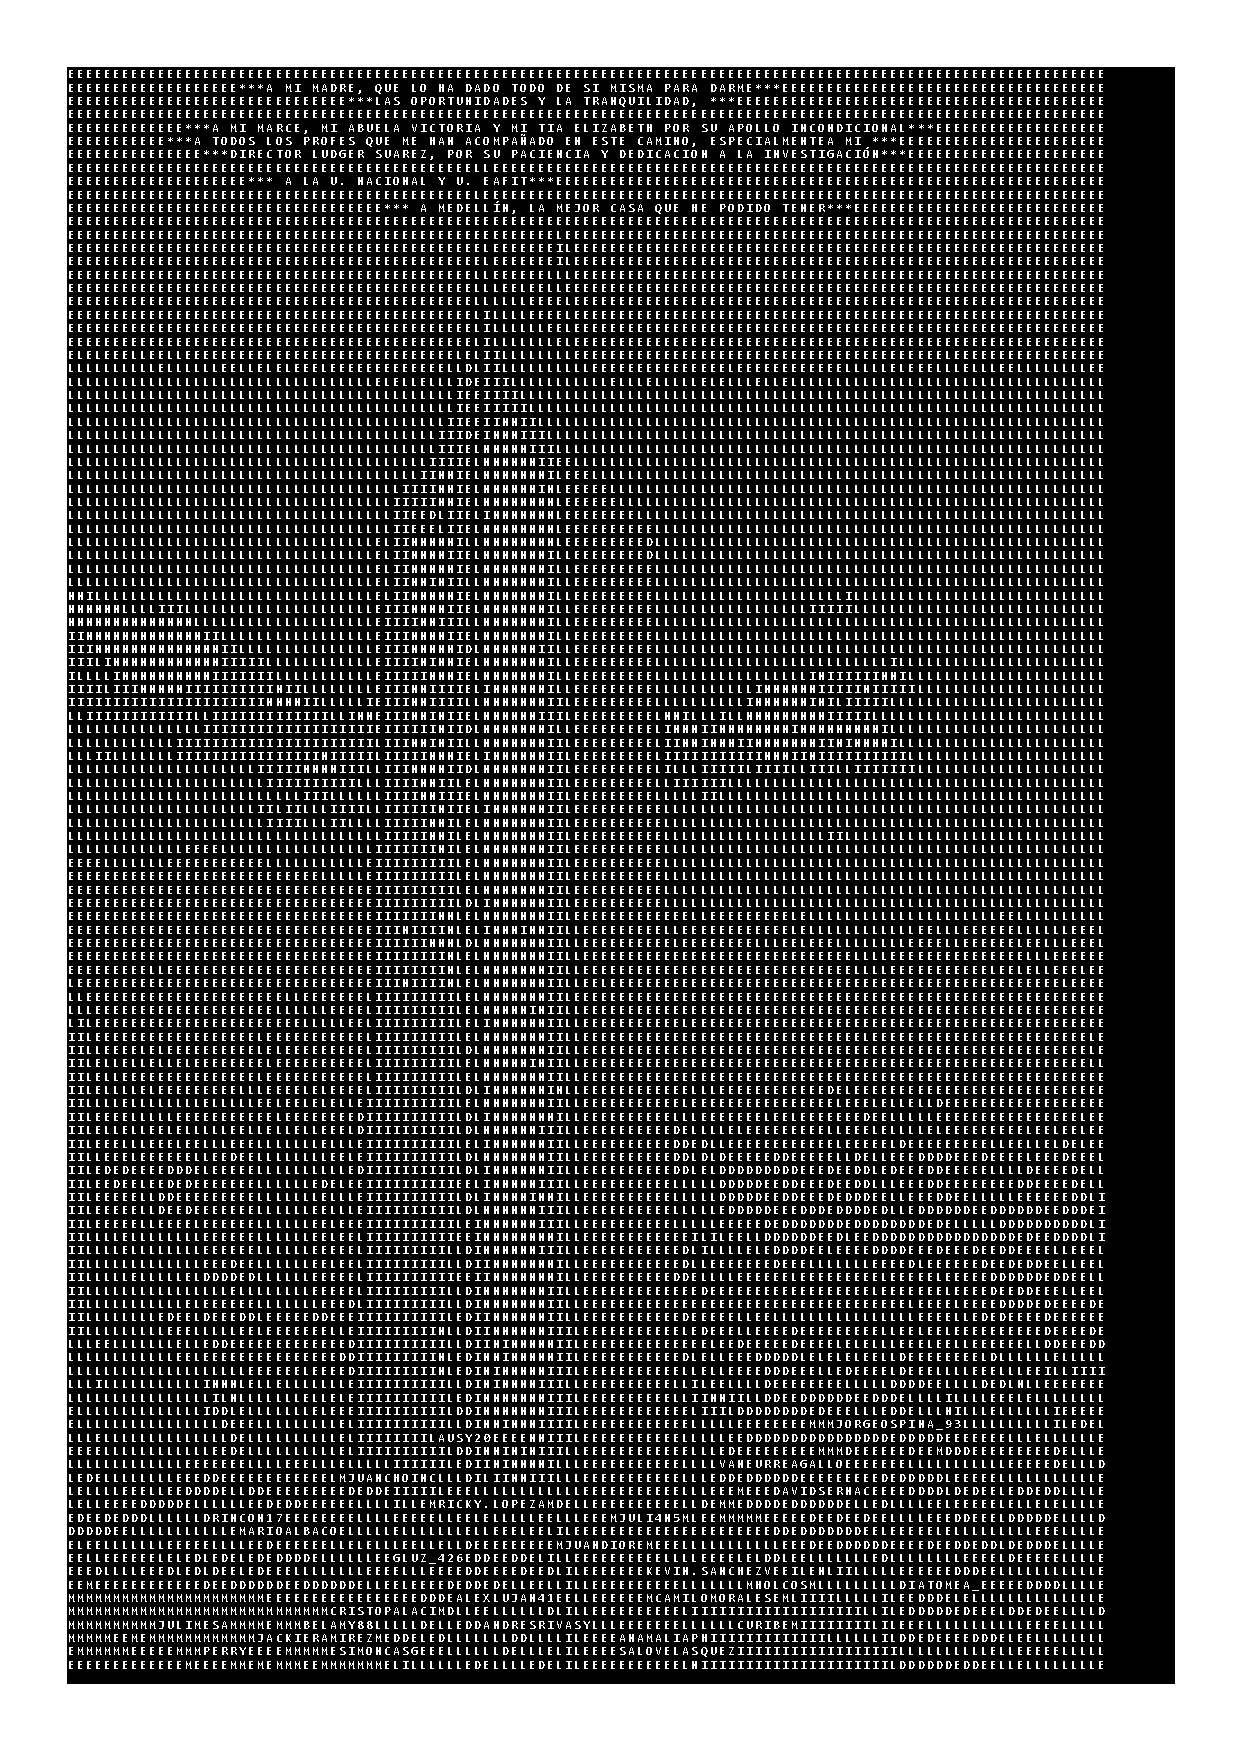
\includegraphics[trim={0 0.1cm 2.2cm 0},clip,scale=0.8]{img/dedicatoria/dedicatoria.pdf}
\end{figure}

\newpage{\pagestyle{empty}\cleardoublepage}

\newpage
\textbf{\LARGE Resumen}\\
En esta investigacion se demuestra la aplicaci\'on de m\'etodos de an\'alisis de equilibrio l\'imite (bishop simplificado), aplicado de manera tridimensional sobre un sector conocido popularmente como Vereda Monteloro, en el municipio de Ciudad Bolivar, Antioquia. Para dicho procedimiento se utilizan como insumos: informaci\'on geogr\'afica y de elevaci\'on contenida en un modelo de elevaci\'on digital(DEM por sus siglas en ingl\'es), par\'ametros de resistencia, espec\'ificamente \'angulo de fricci\'on y cohesion obtenido de ensayos de laboratorio ejecutados sobre muestras recolectadas en la zona de estudio. Como resultado se obtiene un mapa de calor de la zona trabajada en el cual se logra apreciar la distribuci\'on de factores de seguridad y su correlaci\'on con factores como la pendiente y los mismos par\'ametros de resistencia. Adicionalmente se obtiene informacion quantitativa la 

. Se detalla y ejemplifica el uso de Scoops3D como herramienta computacional para la generaci\'on del mapa de distribuciones de factores de seguridad. 
\addcontentsline{toc}{chapter}{\numberline{}Resumen}\\\\
